\documentclass[aspectratio=169, t, 8pt]{beamer}

%------configurando acentos-----------
\usepackage[utf8]{inputenc}
\usepackage[T1]{fontenc}
\usepackage[brazil]{babel}
\usepackage{montserrat}
\usefonttheme[onlymath]{serif}
\usepackage{booktabs} % Tabelas elegantes sem linhas verticais
\usepackage[most]{tcolorbox}

%-------Estilos Beamer---------------
\usetheme{metropolis}
%\usecolortheme{crane}
%\usefonttheme{serif}
\linespread{1.2}

% Personalização de Cores (Exemplo: Minimal Teal)
% Cores Base
\definecolor{BgCanvas}{HTML}{F9F9FB}      % Off-white muito suave
\definecolor{MainText}{HTML}{2B2D42}      % Grafite escuro para alta legibilidade
\definecolor{PrimaryAccent}{HTML}{4A6FA5} % Azul poeira (Dusty Blue)

% Tons Pastéis para Destaques e Cards
\definecolor{PastelGreenBg}{HTML}{E8F0EC}  % Sálvia Claro (Sucesso / Destaque Positivo)
\definecolor{PastelGreenFg}{HTML}{2D5A44}

\definecolor{PastelCoralBg}{HTML}{FDEAE6}  % Coral Soft (Atenção / Problema / Alerta)
\definecolor{PastelCoralFg}{HTML}{7A3025}

\definecolor{PastelPurpleBg}{HTML}{F0EBF4} % Lavanda (Conceitos / Citações)
\definecolor{PastelPurpleFg}{HTML}{4A3E56}

\definecolor{PastelYellowBg}{HTML}{FFF4E6} % Areia / Manteiga (Notas / Dados Secundários)
\definecolor{PastelYellowFg}{HTML}{7A522A}

% --- CONFIGURAÇÕES DE TEMA BEAMER ---
%\usetheme{metropolis}

\setbeamertemplate{itemize item}{\textcolor{MainText}{$\bullet$}}
\setbeamertemplate{itemize subitem}{\textcolor{MainText}{\scriptsize$\circ$}}
\setbeamertemplate{itemize 3rditem}{\textcolor{MainText}{\tiny$\blacksquare$}}

\setbeamercolor{background canvas}{bg=BgCanvas}
\setbeamercolor{normal text}{fg=MainText}
\setbeamercolor{frametitle}{bg=PastelGreenFg, fg=BgCanvas}
\setbeamercolor{title}{fg=MainText}
\setbeamercolor{subtitle}{fg=PrimaryAccent}
\setbeamercolor{structure}{fg=PrimaryAccent}

% Remove a linha amarela padrão do Metropolis sob o título
\setbeamertemplate{title separator}{}
\setbeamertemplate{progress bar in section page}{}

% --- ESTILOS DE CARDS PASTEL COM TCOLORBOX ---
\newtcolorbox{cardverde}[1][]{
  colback=PastelGreenBg,
  colframe=PastelGreenFg,
  coltext=PastelGreenFg,
  arc=6pt,
  boxrule=0pt,
  left=12pt, right=12pt, top=10pt, bottom=10pt,
  fonttitle=\bfseries\small,
  #1
}

\newtcolorbox{cardcoral}[1][]{
  colback=PastelCoralBg,
  colframe=PastelCoralFg,
  coltext=PastelCoralFg,
  arc=6pt,
  boxrule=0pt,
  left=12pt, right=12pt, top=10pt, bottom=10pt,
  fonttitle=\bfseries\small,
  #1
}

\newtcolorbox{cardpurple}[1][]{
  colback=PastelPurpleBg,
  colframe=PastelPurpleFg,
  coltext=PastelPurpleFg,
  arc=6pt,
  boxrule=0pt,
  left=12pt, right=12pt, top=10pt, bottom=10pt,
  fonttitle=\bfseries\small,
  #1
}

\newtcolorbox{cardyellow}[1][]{
  colback=PastelYellowBg,
  colframe=PastelYellowFg,
  coltext=PastelYellowFg,
  arc=6pt,
  boxrule=0pt,
  left=12pt, right=12pt, top=10pt, bottom=10pt,
  fonttitle=\bfseries\small,
  #1
}


%--------Dados do Documento
\title{Matemática: Funções do 2º Grau}
\subtitle{Além da Fórmula de Bhaskara}
\author{prof. Eduardo}
\institute{Pré-Universitário Oficina do Saber / UFF}
\date{\today}


%-------- Pacotes Matemática -------------
\usepackage{amsmath}
\usepackage{amsthm}
\usepackage{amsfonts}
\usepackage{amssymb}
\usepackage{xfrac}
\usepackage{thmtools}

%-------- Configuração Listas---------


%------------- Atalho para imagens ------------
\graphicspath{{./src/img/}}


\begin{document}

    \begin{frame}[plain]
        \titlepage
    \end{frame}

    \begin{frame}[plain]
        \vspace*{\fill}
        \Huge{
            \[
                x = \frac{-b \pm \sqrt{b² - 4 \cdot a \cdot c}}{2 \cdot a}
            \]
        }
        \vspace*{\fill}
    \end{frame}

    \begin{frame}{Afinal, o que representam as Funções do 2º Grau?}
    \vspace{0.2cm}

        Quando pensamos em Funções do 2º, normalmente, nos vem a ideia da fórmula de Bhaskara para encontrarmos suas raízes. Mas é só isso?

        A resposta é \textbf{Não}!

        Funções do segundo grau representam uma importante figura no plano: a \textit{parábola}. Essa curva, para além da importância na Física, é uma importante ferramenta para verificar custos máximos e mínimos, lucro, alacance máximo, entre outras coisas.

        É dessa forma, também que o ENEM nos cobra esse conteúdo.

\vspace{1.7em}
  \begin{columns}[T]
    \begin{column}{0.7\textwidth}
      \begin{cardverde}[title=Bhaskara --- O plano B?]
        \textbf{Sim!} Equações são ferrmentas, seu uso é a segunda etapa de nossa solução. A primeira é entender o que o texto da questão ou o gráfico da função nos diz.
      \end{cardverde}
      
      \vspace{0.3cm}
    \end{column}
    
  \end{columns}
\end{frame}

    \begin{frame}
        \frametitle{Funções}
        \vspace{2em}
            \begin{figure}[!htbp]
                \centering
                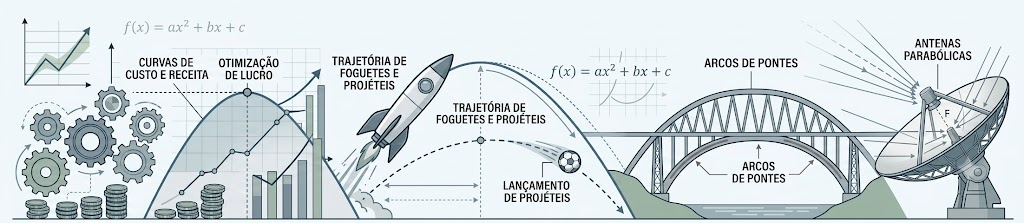
\includegraphics[width=1\textwidth]{slide03_parabola_mundo_real.jpg}  
            \end{figure}
            \vspace{1em}
            \begin{columns}[T]
                \begin{column}{0.6\textwidth}
                    \begin{center}
                        Então, o jogo vai ser ler e compreender o texto e o gráfico e saber relacionar com a equação, para procurarmos o que se deseja.
                    \end{center}
                \end{column}
            \end{columns}
    \end{frame}    

    \begin{frame}
        \frametitle{Entendendo a Equação do 2º Grau}
       
        \begin{columns}[T]
            \begin{column}{0.35\textwidth}
                \begin{figure}[!htbp]
                    \centering
                    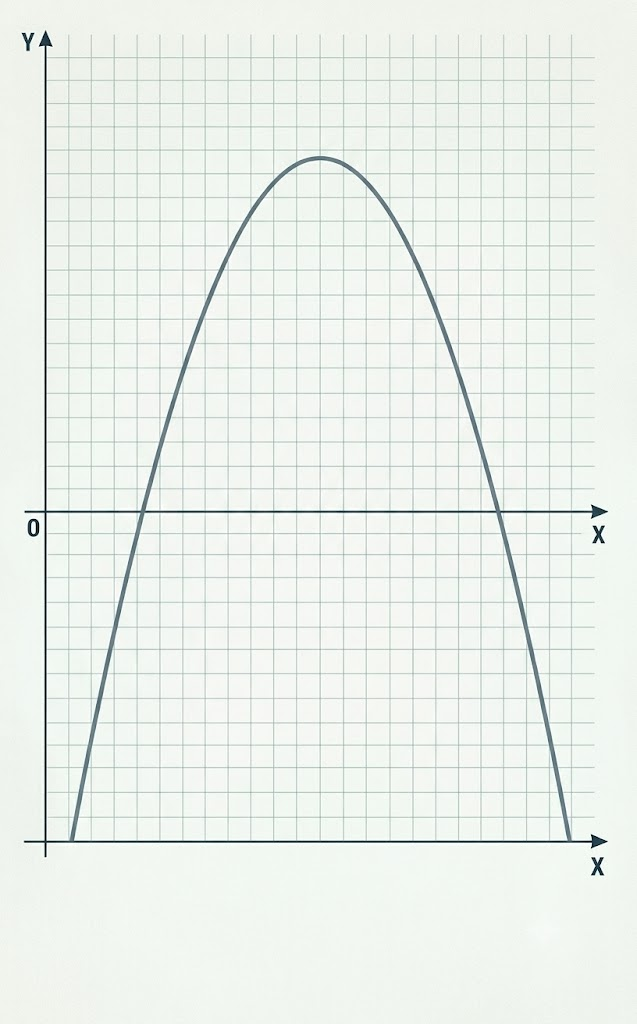
\includegraphics[width=1.1\textwidth]{slide04_parabola_plano_cartesiano.jpg}
                \end{figure}
            \end{column}
            \begin{column}{0.6\textwidth}
                {\huge
                \begin{equation*}
                    f(x) = ax^2 +bx + c
                \end{equation*}
                }
                \vspace{-.3em}
                \begin{cardyellow}[title=O Coeficiente \large $a$]
                    \begin{itemize}
                        \item Quando o coeficiente $a$ é positivo ($a>0$), a função tem um \textbf{teto}
                        \item Quando o coeficiente $a$ é negativo ($a<0$), a função tem um \textbf{piso}
                    \end{itemize}
                \end{cardyellow}

                \begin{cardpurple}[title=O Coeficiente \large $c$]
                     \begin{itemize}
                        \item Obtemos $f(x)=c$, quando $x=0$. Logo, $(0,c)$ é o ponto em que a curva corta o eixo $y$
                        \item Na maioria das questões representará o valor \textit{inicial}
                    \end{itemize}
                \end{cardpurple}
            \end{column}
        \end{columns}
    \end{frame}

    \begin{frame}
        \frametitle{Os Zeros da Função}

        Aqui utilizamos a tradicional fórmula de Bhaskara. Lembre-se que, do ponto de vista gráfico, os \textit{zeros} da função são os pontos em que a curva corta o eixo $x$.
        
        
        \begin{columns}
            \begin{column}{0.55\textwidth}
                \vfil
                As coordenadas das raízes da função são, portanto, $(x_1,0)$ e $(x_2, 0)$. Para encontrarmos os valores de $x_1$ e $x_2$, utilizamos a famosa fórmula da Bhaskara:

                \[
                x = \frac{-b \pm \sqrt{b^2 - 4 \cdot a \cdot c}}{2 \cdot a}
                \]

                \vspace{1em}
                Também podemos calcular as raízes de uma função do segundo grau pelas fórmulas da soma e do produto:

                \begin{columns}
                    
                    \begin{column}{.5\textwidth}
                        \[
                            x_1 + x_2 = \frac{-b}{a}
                            \]    
                        \end{column}
                        
                        \begin{column}{.5\textwidth}
                            \[
                                x_1 \cdot x_2 = \frac{c}{a}
                                \]    
                            \end{column}
                \end{columns}
            
                \vspace{1em}
                Em uma situação problema do ENEM, as raízes podem ter a ver, por exemplo com o momento em que um projétil toca o chão.

            \end{column}
            \begin{column}{0.4\textwidth}
                \begin{figure}
                    \centering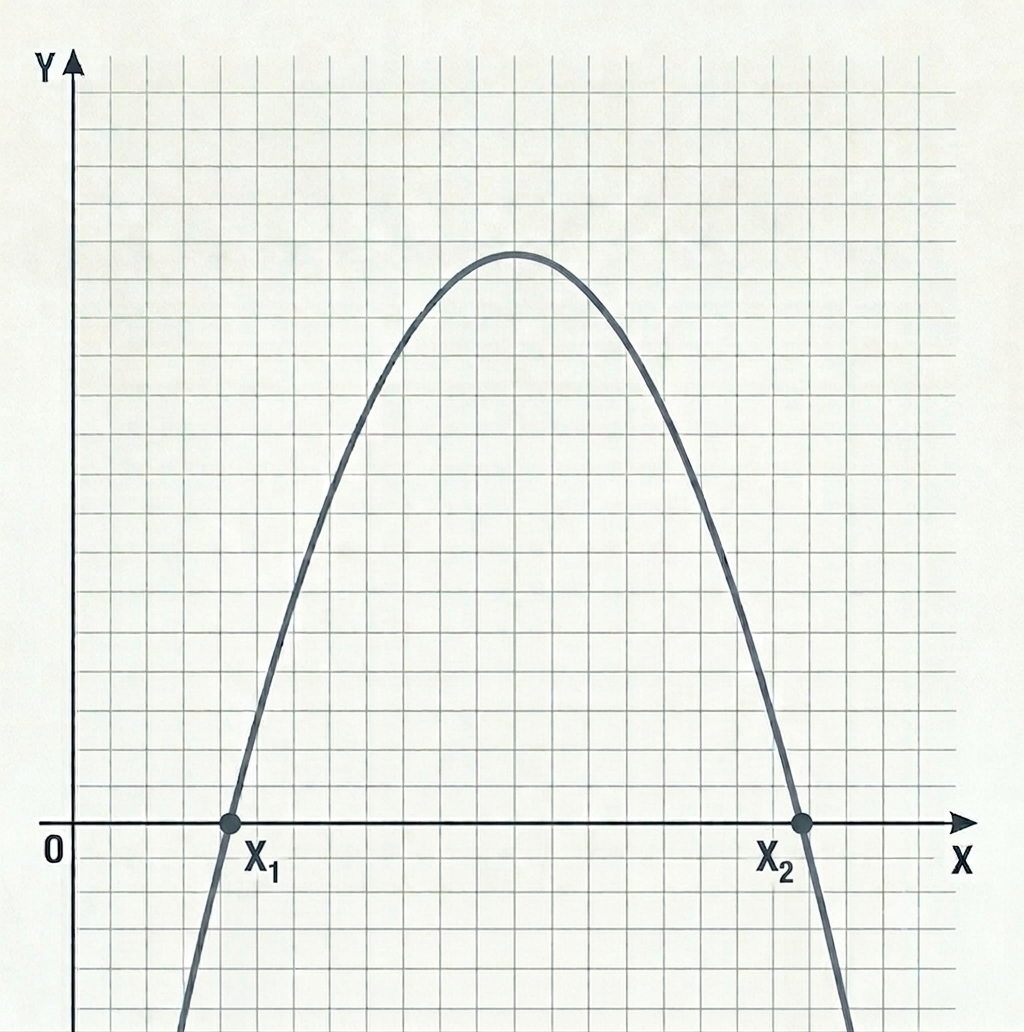
\includegraphics[width=1\textwidth]{slide06_raizes.png}
                \end{figure}
            \end{column}
        \end{columns}
    \end{frame}

    \begin{frame}
        \frametitle{O Vértice: Ponto de virada}

        O vértice é o ponto onde a curva muda o sentido de crescimento. Então, podemos entendê-lo como o ponto mais alto ou mais baixo da parábola --- dependendo do sinal de $a$.

        \begin{columns}
            \begin{column}{0.35\textwidth}
                \begin{figure}[!htbp]
                    \centering
                    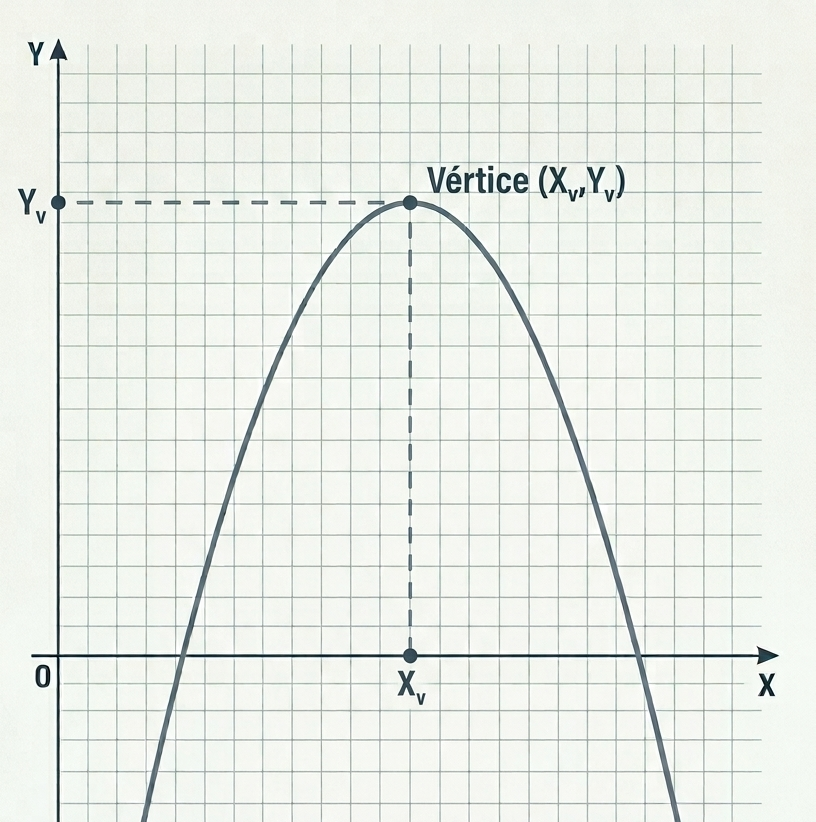
\includegraphics[width=1.1\textwidth]{slide05_vertices.png}
                \end{figure}
            \end{column}
            \begin{column}{0.6\textwidth}
                \vfil
                A coordenada $x$ do vértice de uma parábola é dadas por:
                \begin{cardcoral}[title=Coordenada \large$x$]
                    $x_v = \frac{-b}{2a}$
                    \vspace{13em}
                \end{cardcoral}
                
            \end{column}
        \end{columns}
    \end{frame}

    \begin{frame}
        \frametitle{O Vértice: Ponto de virada}

        A coordenada $y$ do vértice da parábola será determinada a partir da substituição da sua coordenada $x$, na equação da parábola.

        \begin{columns}
            \begin{column}{0.35\textwidth}
                \begin{figure}[!htbp]
                    \centering
                    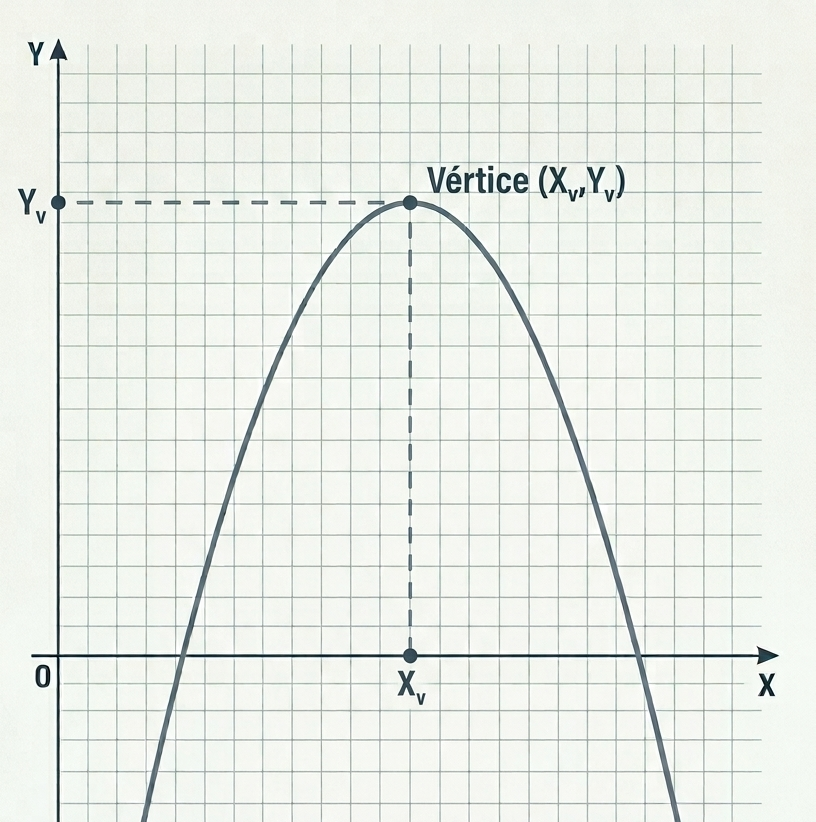
\includegraphics[width=1.1\textwidth]{slide05_vertices.png}
                \end{figure}
            \end{column}
            \begin{column}{0.6\textwidth}
                \vfil
                \begin{cardverde}[title=Coordenada \large$y$]
                    \begin{columns}                        
                        \begin{column}{.4\textwidth}
                            $y_v = \frac{-\Delta}{4a}$
                        \end{column}
                        \begin{column}{.4\textwidth}
                            \small Lembrando que $\Delta = b^2 - 4\cdot a \cdot c$
                        \end{column}
                    \end{columns}
                    \vspace{6.5em}
                \end{cardverde}
                \begin{cardpurple}[title=Lembre-se!]
                    O vértice é o ponto mais alto (máximo) ou mais baixo (mínimo) do gráfico.
                \end{cardpurple}
            \end{column}
        \end{columns}
    \end{frame}

    \begin{frame}
        \frametitle{Jogando o jogo do ENEM}
        \begin{table}
            \centering
            \setlength{\tabcolsep}{0.07\textwidth}
            \begin{tabular}{p{.25\textwidth} p{.2\textwidth} p{.15\textwidth}}
                \textbf{Enunciado} & \textbf{O que se pede?} & \textbf{Que Fórmula?}\\
                \hline\\
                \textit{Qual a \textbf{quantidade} de peças para maximizar o lucro?} & A coordenada $x$ do vértice & $x_v = \frac{-b}{2a}$
                \vspace{0.8cm}\\
                
                \hline\\

                \textit{Qual o \textbf{valor} do lucro máximo?} & A coordenada $y$ do vértice & $y_v = \frac{-\Delta}{4a}$
                \vspace{0.8cm}\\
                
                \hline\\

                \textit{Em quanto \textbf{tempo} o objeto alcança a altura máxima?} & A variável intependente ($x$), no vértice do gráfico & $x_v = \frac{-b}{2a}$
                \vspace{0.8cm}\\
                
                \hline\\

                \textit{Qual foi a \textbf{altura máxima} atingida pelo objeto} & O valor máximo no eixo $y$ & $\displaystyle y_v = \frac{-\Delta}{4a}$
                \vspace{0.8cm}\\
                
                \hline\\
            \end{tabular}
        \end{table}
    \end{frame}
\end{document}